\documentclass[8pt,red]{beamer}
\usepackage{amsmath,amsthm,amsfonts,amssymb,amsbsy}
\usepackage{stmaryrd} 
\usepackage{subeqnarray}
\usepackage{cases}
\usepackage{pifont}
\usepackage{fancyhdr}
\usepackage{lastpage}
\usepackage{graphicx}
\usepackage{subfloat}
\usepackage{rotating}
\usepackage{tikz}
\setbeamertemplate{theorem}[ams style]
\setbeamertemplate{theorems}[numbered]
\setbeamerfont{framesubtitle}{size=\Large}

\usepackage{algpseudocode,algorithm}
\usepackage[square,sort&compress,numbers]{natbib}
\usepackage{type1cm}
\usepackage{mathtools}\mathtoolsset{showonlyrefs=false}
\usepackage{subcaption}
\newcommand{\memo}[1]{\textbf{[MEMO:} #1 \ \textbf{ : end memo] }}
\newcommand{\OMIT}[1]{\textbf{[OMIT:} #1 \ \textbf{ --- end OMIT] }}
\newcommand{\Authornote}{\renewcommand{\thefootnote}{\fnsymbol{footnote}}}
\newcommand{\authornote}{\Authornote\footnote}
%\setlength{\topmargin}{-14mm}
%\setlength{\oddsidemargin}{-2mm}
%\setlength{\textwidth}{166mm}
%\setlength{\textheight}{50\baselineskip}
%\addtolength{\textheight}{\topskip}
\renewcommand{\baselinestretch}{1.2}
\setlength{\parskip}{0.0pt}
\renewcommand{\topfraction}{0.9}
\renewcommand{\bottomfraction}{0.9}
\renewcommand{\dbltopfraction}{0.9}
\renewcommand{\textfraction}{0.1}
\renewcommand{\floatpagefraction}{0.9}
\renewcommand{\dblfloatpagefraction}{0.9}
\setcounter{topnumber}{3}
\setcounter{bottomnumber}{3}
\setcounter{totalnumber}{3}
\theoremstyle{plain}
\newtheorem{assumption}[theorem]{Assumption}
\theoremstyle{definition}
\newtheorem{proposition}[theorem]{命題}
\theoremstyle{remark}
\newtheorem{remark}[theorem]{Remark}
\newcommand{\refalg}[1]{Algorithm~\ref{#1}}
\newcommand{\refrem}[1]{Remark~\ref{#1}}
\newcommand{\reffig}[1]{Figure~\ref{#1}}
\newcommand{\reftab}[1]{Table~\ref{#1}}
\newcommand{\finbox}{\nolinebreak\hfill{\small $\blacksquare$}}
\newcommand{\MIN}{\mathop{\mathrm{Minimize}}}
\newcommand{\MAX}{\mathop{\mathrm{Maximize}}}
\newcommand{\Min}{\mathop{\mathrm{minimize}}}
\newcommand{\st}{\mathop{\mathrm{s.{\,}t.}}}
\newcommand{\ST}{\mathop{\mathrm{subject~to}}}
\newcommand{\sign}{\mathop{\mathrm{sgn}}\nolimits}
\newcommand{\domain}{\mathop{\mathrm{dom}}\nolimits}
\newcommand{\rank}{\mathop{\mathrm{rank}}\nolimits}
\newcommand{\boundary}{\mathop{\mathrm{bd}}\nolimits}
\newcommand{\diag}{\mathop{\mathrm{diag}}\nolimits}
\newcommand{\tr}{\mathop{\mathrm{tr}}\nolimits}
\newcommand{\prox}{\mathop{\boldsymbol{\mathrm{prox}}}\nolimits}
\newcommand{\argmin}{\operatornamewithlimits{\mathrm{arg\,min}}}
\newcommand{\argmax}{\operatornamewithlimits{\mathrm{arg\,max}}}
\newcommand{\overRe}{\ensuremath{\Re\cup\{+\infty\}}}
\renewcommand{\Re}{\ensuremath{\mathbb{R}}}
\newcommand{\bi}[1]{\ensuremath{\boldsymbol{#1}}}
\newcommand{\rr}[1]{\ensuremath{\mathrm{#1}}}
\newcommand{\bs}[1]{\ensuremath{\boldsymbol{\mathsf{#1}}}}
\newcommand{\LC}{\ensuremath{\mathcal{L}}}
\usepackage{color}
\newcommand{\commentva}[1]{\textcolor{blue}{#1}}


%\input{../macro-mjean.tex}
% %hideothersubsections
% \usetheme[hideothersubsections,width=2.5cm]{Goettingen}
% %\useoutertheme[headline=empty]{miniframes}

\usetheme[]{Montpellier}
\makeatletter
\useoutertheme[height=0pt, width=0cm]{sidebar}
{\usebeamercolor{structure}}
\setbeamertemplate{sidebar canvas \beamer@sidebarside}[vertical shading][top=structure.fg!25,bottom=structure.fg!10]

%%% Local Variables: 
%%% mode: latex
%%% TeX-master: t
%%% End: 


\title{Alternating Direction Method of Multipliers (ADMM) for Frictional Contact}
\author{Vincent Acary, Yoshiro Kanno \& Nicolas Molina}
\date{\today }

\setbeamertemplate 
{footline} 
{\quad\hfill\strut\insertsection\quad--\quad\insertframenumber/\inserttotalframenumber\strut\quad\quad} 

\graphicspath{{../figure/}{./figure-monopoli/}{/Users/acary/Work/faf/TeX/figure/},{./figure}}

\begin{document}

{
\frame{\titlepage
  \begin{center}
    
\includegraphics[width=0.3\textwidth]{logo-inria-chile-small.png}
  \end{center}
  $$ $$
}
}

\begin{frame}
\frametitle{Outline}
\small 
\tableofcontents[hideallsubsections]
\end{frame}

\AtBeginSection[]
{
  \begin{frame}{Outline}
  	\small 
    \tableofcontents[currentsection,hideallsubsections]
  \end{frame}
}

\section{Introduction}
\begin{frame}{Finite-dimensional frictional contact problem}
The problem in \citep{Acary2013} reads:
\begin{align}
	\begin{cases}
	M \bi{v} + \bi{f} = H^{\top} \bi{r}  \\
	K_{e,\mu}^{*}\ni \tilde{\bi{u}} \perp \bi{r} \in K_{e,\mu} \\
	\end{cases}
	\begin{array}{l}
	\bi{u} := H \bi{v} + \bi{w} \\
	\tilde{\bi{u}} := \bi{u} + \Phi(\bi{u})
	\end{array}
	\label{CF.complementary}
\end{align}
The problem data are:
\begin{itemize}
\item $M \in \Re^{n \times n}$, a positive definite matrix 
\item $f \in \Re^{n}$
\item $H \in \Re^{n \times m}$, with $m = 3n_{c}$, $n_{c}$ number of contacts
\item $w \in \Re^{m}$
\item $\mu \in \Re^{n_{c}}$, a vector of coefficients of friction 
\end{itemize}
The unknowns are two vectors:
\begin{itemize}
\item $v \in \Re^{n}$, a velocity-like vector
\item $r \in \Re^{m}$, a contact reaction or impulse
\end{itemize}
\end{frame}

\begin{frame}{Finite-dimensional frictional contact problem}
The set $K_{e,\mu} \subseteq \Re^{m}$ is the cartesian product of Couloumb's friction second-order cone at each contact and $K_{e,\mu}^{*}$ its dual cone, i.e.,
\begin{align}
	K_{e,\mu} = \prod_{\alpha = 1...n_{c}} K_{e,\mu}^{\alpha} =
	\prod_{\alpha = 1...n_{c}} \{ (x_{1},\bi{x}_{2}) \in \Re \times \Re^{n-1} \mid \| \bi{x}_{2} \| \le \mu x_{1} \}
\end{align}
where $x_{1} = \bi{x}^{\top} e$, $\bi{x}_{2} = \bi{x} - x_{1} e$ and $K_{e,\mu}^{*} =  K_{e,\frac{1}{\mu}}$. The function $\Phi: \Re^{m} \rightarrow \Re^{m}$ is a nonsmooth function defined as
\begin{align}
	\Phi(\bi{u}) = [\mu^{\alpha} \| E_{t} \bi{u}^{\alpha} \| \hat{\bi{e}}_{n}, \alpha = 1...n_{c}]^{\top}
\end{align}
where $\hat{\bi{e}}_{t} = [1, 0, 0]^{\top}$ is the normal component vector and $E_{t} = \diag (0,1,1) \in \Re^{3 \times 3}$ the linear transformation that maps to the tangential part of $\tilde{\bi{u}}$.
\end{frame}

\section{ADMM method}

\subsection{Fundamentals}

\begin{frame}{Fundamentals}
Let $f : \Re^{n} \to \overRe$ and 
$g : \Re^{m} \to \overRe$ be a closed proper convex 
functions. 
Consider the following convex optimization problem in variables 
$\bi{x} \in \Re^{n}$ and $\bi{y} \in \Re^{m}$: 
\begin{subequations}\label{P.convex.1}%
  \begin{alignat}{3}
    & \MIN  &{\quad}& 
    f(\bi{x}) + g(\bi{y}) \\
    & \ST && 
    A \bi{x} + B \bi{y} = \bi{c}  
  \end{alignat}
\end{subequations}
where $A \in \Re^{l \times n}$ and $B \in \Re^{l \times m}$ are constant 
matrices, and $\bi{c} \in \Re^{l}$ is a constant vector.
\end{frame}

\begin{frame}{Fundamentals}
The augmented Lagrangian of problem \eqref{P.convex.1} is defined as 
\begin{align}
  L_{\rho}(\bi{x};\bi{y};\bi{w}) 
  = f(\bi{x}) + g(\bi{y}) 
  + \bi{w}^{\top} (A \bi{x} + B \bi{y} - \bi{c}) 
  + \frac{\rho}{2} \| A \bi{x} + B \bi{y} - \bi{c} \|^{2} 
  \label{eq.ADMM.Lagrangian.1}
\end{align}
where $\rho > 0$ is the penalty parameter, 
and $\bi{w} \in \Re^{l}$ is the Lagrange multiplier (or the dual 
variable). 
ADMM consists of the iterations 
\begin{align}
  \bi{x}^{k+1} 
  &:= \argmin_{\bi{x}} L_{\rho}(\bi{x};\bi{y}^{k};\bi{w}^{k}) \\
  \bi{y}^{k+1} 
  &:= \argmin_{\bi{y}} L_{\rho}(\bi{x}^{k+1};\bi{y};\bi{w}^{k}) \\
  \bi{w}^{k+1} 
  &:= \bi{w}^{k} 
  + \rho (A \bi{x}^{k+1} + B \bi{y}^{k+1} - \bi{c}) 
\end{align}
where the dual variable is updated via dual ascent method.
\end{frame}

\begin{frame}{Fundamentals}
ADMM is often described in a slightly different form. 
Define $\bi{z}$ by $\bi{z} = \bi{w} / \rho$. 
Then the augmented Lagrangian in \eqref{eq.ADMM.Lagrangian.1} is reduced 
to 
\begin{align}
  L_{\rho}(\bi{x};\bi{y};\bi{z}) 
  = f(\bi{x}) + g(\bi{y}) 
  + \frac{\rho}{2} \| A \bi{x} + B \bi{y} - \bi{c} + \bi{z} \|^{2} 
  - \frac{\rho}{2} \| \bi{z} \|^{2} .
  \label{eq.ADMM.Lagrangian.2}
\end{align}
Using $L_{\rho}$ in \eqref{eq.ADMM.Lagrangian.2}, we can express ADMM as 
follows: 
\begin{align}
  \bi{x}^{k+1} 
  &:= \argmin_{\bi{x}} L_{\rho}(\bi{x};\bi{y}^{k};\bi{z}^{k}) , 
  \label{eq.ADMM.update.2.1} \\
  \bi{y}^{k+1} 
  &:= \argmin_{\bi{y}} L_{\rho}(\bi{x}^{k+1};\bi{y};\bi{z}^{k}) , 
  \label{eq.ADMM.update.2.2} \\
  \bi{z}^{k+1} 
  &:= \bi{z}^{k} + A \bi{x}^{k+1} + B \bi{y}^{k+1} - \bi{c} 
  \label{eq.ADMM.update.2.3}
\end{align}
The expression in \eqref{eq.ADMM.update.2.1}, \eqref{eq.ADMM.update.2.2}, 
and \eqref{eq.ADMM.update.2.3} is called the ADMM in the scaled form, 
and $\bi{z}$ is called the scaled dual variable.
\end{frame}

\subsection{Stop criterion}
\begin{frame}{Stop criterion}
The residuals of the optimality conditions can be related to an approximated bound:
\begin{align}
\begin{array}{l}
  \| \bi{r}^{k} \| \leq \epsilon^{pri} \\
  \| \bi{s}^{k} \| \leq \epsilon^{dual}  
\end{array} \label{eq.stopcriterion}
\end{align}
where $\bi{r}^{k+1} = A \bi{x}^{k+1} + B \bi{y}^{k+1} - \bi{c}$ and $\bi{s}^{k+1} = \rho A^{T} B \left( \bi{y}^{k+1} - \bi{y}^{k} \right)$ are the primal and dual residuals, respectively; and $\epsilon^{pri} > 0$ and $\epsilon^{dual} > 0$ are feasibility tolerances for the primal and dual residuals. These tolerances can be choosen using an absolute and relative criterion, such as
\begin{align}
\begin{array}{l}
  \epsilon^{pri} = \sqrt{l} \epsilon^{abs} + \epsilon^{rel} \max \lbrace \|A \bi{x}^{k+1}\|,\|B \bi{y}^{k+1}\|, \|\bi{c}\|  \rbrace \\
  \epsilon^{dual} = \sqrt{n} \epsilon^{abs} + \epsilon^{rel} \|A^{T} \rho \bi{z}^{k+1}\| 
\end{array}
\end{align}
where $\epsilon^{abs} > 0$ and $\epsilon^{rel} > 0$ is an absolute and relative tolerance, respectively. This values typically depend on the scale of the data size.
\end{frame}

\section{ADMM formulation of problem}

\subsection{Coulomb friction problem via convex optimization}
\begin{frame}{Coulomb friction problem via convex optimization}
In \citep{acary2011formulation}, a parametric convex optimization formulation is presented for the dynamical Coulomb friction problem. The problem reads 
\begin{subequations}\label{P.original.friction.SOCP.1}%
  \begin{alignat}{3}
    & \MIN_{\bi{v}, \tilde{\bi{u}}}  &{\quad}& 
    \frac{1}{2} \bi{v}^{\top} M \bi{v} + \bi{f}^{\top} \bi{v} \\
    & \ST && 
    \tilde{\bi{u}} = H \bi{v} + \bi{w} + \Phi(\bi{s})  \\
    & && 
    \tilde{\bi{u}} \in K_{e,\mu}^{*} 
  \end{alignat}
\end{subequations}
where $\bi{s} \in \Re^{m}$ is a parameter vector and $\Phi(\bi{s}) = [\mu^{\alpha} \| E_{t} \bi{s}^{\alpha} \| \hat{e}_{n}, \alpha = 1...n_{c}]^{\top}$. 
\end{frame}
%Lower proper convex function: we remove the conic constraint but the trade off is to have an objective function non-smooth (that's why we use subgradients)

\begin{frame}{Coulomb friction problem via convex optimization}
Let $\delta_{K_{e,\mu}^{*}} : \Re^{n} \to \overRe$ denote the 
indicator function of $K_{e,\mu}^{*}$, i.e., 
\begin{align}
  \delta_{K_{e,\mu}^{*}}(\bi{x}) = 
  \begin{dcases*}
    0 
    & if $\bi{x} \in K_{e,\mu}^{*}$ \\
    +\infty
    & otherwise. 
  \end{dcases*}
\end{align}
Then problem \eqref{P.original.friction.SOCP.1} is equivalently rewritten as follows:
 \begin{subequations}\label{P.quadratic.SOCP.2}%
   \begin{alignat}{3}
     & \MIN_{\bi{v}, \tilde{\bi{u}}}  &{\quad}& 
    \frac{1}{2} \bi{v}^{\top} M \bi{v} + \bi{f}^{\top} \bi{v} + \delta_{K_{e,\mu}^{*}}(\tilde{\bi{u}}) \\
     & \ST & & 
     \tilde{\bi{u}} = H \bi{v} + \bi{w} + \Phi(\bi{s})   
   \end{alignat}
 \end{subequations}  
\end{frame}

\subsection{Iterations}
\begin{frame}{Iterations}
Problem \eqref{P.quadratic.SOCP.2} is a minimization problem of a convex 
function under linear equality constraints. 
Its augmented Lagrangian (in the scaled form) is formulated as 
\begin{align}
  L_{\rho}(\bi{v};\tilde{\bi{u}};\bi{\zeta}) 
  =& \frac{1}{2} \bi{v}^{\top} M \bi{v} + \bi{f}^{\top} \bi{v} 
  +  \delta_{K_{e,\mu}^{*}}(\tilde{\bi{u}}) +  \frac{\rho}{2} 
  \| H \bi{v} + \bi{w} + \Phi(\bi{s}) + \bi{\zeta}  - \tilde{\bi{u}} \|^{2}
    - \frac{\rho}{2} \| \bi{\zeta}\|^{2} 
    \label{eq.ADMM.friction.AugLagrange}
\end{align}
where $\rho$ is the penalty parameter, and $\bi{\zeta} \in \Re^{m}$ is  the scaled dual variable (the scaled Lagrange multiplier). 
The ADMM solving problem \eqref{P.quadratic.SOCP.2} consists of 
iterating the updates (see \eqref{eq.ADMM.update.2.1}, 
\eqref{eq.ADMM.update.2.2}, and \eqref{eq.ADMM.update.2.3}) 
\begin{align}
  \bi{v}^{k+1} 
  &:= \argmin_{\bi{v}} 
  L_{\rho}(\bi{v};\tilde{\bi{u}}^{k};\bi{\zeta}^{k})  
  \label{eq.ADMM.friction.1.1} \\
  \tilde{\bi {u}}^{k+1}
  &:= \argmin_{\tilde{\bi{u}}} 
    L_{\rho}(\bi{v}^{k+1};\tilde{\bi{u}};\bi{\zeta}^{k}) 
    \label{eq.ADMM.friction.1.2} \\
  \bi{\zeta}^{k+1} &:= \bi{\zeta}^{k} 
  + 
  H \bi{v}^{k+1} +\bi{w} +\Phi(\bi{s}) - \tilde{\bi{u}}^{k+1}  
  \label{eq.ADMM.friction.1.3}
\end{align}

%Precursors: dual ascent method (gradient ascent, opposite to the gradient descent method with a step size) and dual decomposition, augmented lagrangians and the method of multipliers (version of dual ascent method)
\end{frame}

\begin{frame}{Iterations}

\begin{itemize}
\item $v$-update
\end{itemize}
The first step in \eqref{eq.ADMM.friction.1.1} corresponds to the solution to the following linear system: 
\begin{align}
  \Bigl[ M + 
  \rho H^{\top} H \Bigr] \bi{v}^{k+1} 
  = -\bi{f} 
  + \rho H^{\top} (\tilde{\bi{u}}^k - \bi{w} - \Phi(\bi{s}) - \bi{\zeta}^k)   \label{eq.ADMM.friction.2.1}
\end{align}

\begin{itemize}
\item $\tilde{u}$-update
\end{itemize}
The second step in \eqref{eq.ADMM.friction.1.2} can be computed independently for each $\alpha = 1 ... n_{c}$ as 
\begin{align}
  \tilde{\bi{u}}^{k+1}
  &:= \argmin_{\tilde{\bi{u}}} 
    \delta_{K_{e,\mu}^{*}}(\tilde{\bi{u}}) 
    + \frac{\rho}{2} 
    \| H \bi{v}^{k+1} + \bi{w} + \Phi(\bi{s}) + \bi{\zeta}^{k} - \bi{\tilde u} \|^{2}
  \label{eq.ADMM.friction.2.2}
\end{align}
which is identified as the proximity operator or the Moreau-Yosida regularization of $\delta_{K_{e,\mu}^{*}}(\tilde{\bi{u}})$ and this can be written explicitly by using the projection onto the second-order cone as
\begin{align}
  \tilde{\bi{u}}^{k+1} := \Pi_{K_{e,\mu}^{*}}(H \bi{v}^{k+1} + \bi{w} + \Phi(\bi{s}) + \bi{\zeta}^{k})
  \label{eq.ADMM.friction.2.2bi}
\end{align}

\end{frame}

%\begin{frame}{Iterations}
%It is recognized in \eqref{eq.ADMM.friction.2.2bi} the fixed-point iteration solution of the VI formulation of \eqref{CF.complementary}, described by Acary in \citep{acary:hal-01630836}, which is related to the zeroes of the natural map, i.e.,
%\begin{align}
%F_{\rho}^{nat}(\tilde{\bi{u}}) = \tilde{\bi{u}} - \Pi_{K_{e,\mu}^{*}}(\tilde{\bi{u}} - \rho \bi{r}) = 0 \label{eq.ADMM.naturalmap}
%\end{align}
%where $\bi{r}$ is the contact reaction or impulse (see Appendix C for the relationship between $\bi{r}$ and $\bi{\zeta}$). This formulation helps us to notice the fixed-point interation for the VI formulation immersed in the ADMM algorithm.
%
%Finally, it is worthy to note that for \eqref{eq.ADMM.friction.2.1} we carry out a Cholesky or LU factorization and \eqref{eq.ADMM.friction.2.2bi} can be solved explicitly by using the formulan given in the next section.
%\end{frame}

\subsection{Projection onto dual second-order cone}
\begin{frame}{Projection onto dual second-order cone}
The projection of $\bi{x}$ onto $K_{e,\mu}^{*}$ could be written as follows
\begin{align}
  \Pi_{K_{e,\mu}^{*}}(\bi{x}) = 
  \begin{dcases*}
	0
    & if $-\bi{x} \in K_{e,\mu}$ \\
    \bi{x}
    & if $\bi{x} \in K_{e,\mu}^{*}$ \\
    \frac{\mu^{2} \left(x_{1} + \frac{1}{\mu} \| \bi{x}_{2} \|\right)}{1+\mu^{2}} 
    \begin{bmatrix}
      1 \\    \frac{1}{\mu} \bi{x}_{2} / \| \bi{x}_{2} \| 
    \end{bmatrix}
    & if $-\bi{x} \not\in K_{e,\mu} \wedge \bi{x} \not\in K_{e,\mu}^{*}$, \\
  \end{dcases*}  
\end{align}
%\begin{itemize}
%\item Finally, it is worthy to note that for \eqref{eq.ADMM.friction.2.1} we carry out a Cholesky or LU factorization and \eqref{eq.ADMM.friction.2.2bi} can be solved explicitly by using the formulan given above.
%\end{itemize}
\end{frame}

\section{Penalty parameter}
%The ADMM technique is surprisingly robust to poorly selected algorithm parameters: under mild conditions, the method is guaranteed to convergence for all positive values of $\rho$ \citep{boyd2011distributed, deng2016global, eckstein2012augmented}. However, a key ingredient in the efficiency and the convergence time of ADMM is the choise of the sequence $\lbrace \rho_{k} \rbrace$. A sensible work has been done in the literature mainly motivated by the rate of convergence. This section presents the most popular approach for choosing the sequence $\lbrace \rho_{k} \rbrace$ for QPs.

\subsection{Optimal penalty parameter selection}
\begin{frame}{Optimal penalty parameter selection}
%In this section we present two main results that have been proposed for QPs in the initial guess of the parameter and we define another two ones.
\begin{itemize}
\item Ghadimi
\item Di Cairano
\item Acary
\item Normal
\end{itemize}
\end{frame}

\begin{frame}{Optimal penalty parameter selection}

\begin{itemize}
\item Ghadimi
\end{itemize}
The $\rho^{\star}$ that minimizes the rate of convergence is
\begin{align}
  \rho^{\star} := \left(\sqrt{\lambda_{min}(H M^{-1} H^{\top}) \lambda_{max}(H M^{-1} H^{\top})}\right) ^{-1} 
\end{align}
If the constraint matrix $H$ is not full rank, the smallest non-zero eigenvalue is taken, which still works as a heuristic to reduce the rate of convergence \citep{ghadimi2015optimal}. It is worth noting that the matrix $H M^{-1} H^{\top}$ is called \textit{Delassus Matrix} and is denoted by $W$.

\begin{itemize}
\item Di Cairano
\end{itemize}
The $\rho^{\star}$ that minimizes the rate of convergence is
\begin{align}
  \rho^{\star} := \sqrt{\lambda_{min}(M) \lambda_{max}(M)}
\end{align}
In this case, the nullity of H equal to zero is avoided \citep{raghunathan2014alternating}.
\end{frame}

\begin{frame}{Optimal penalty parameter selection}

\begin{itemize}
\item Acary
\end{itemize}
In this report is proposed the following value, where the penalty parameter could be seen as the factor that balance the matrix involved in the the first term of \eqref{eq.ADMM.friction.2.1}
\begin{align}
  \rho^{\star} := \frac{\Vert M \Vert_{1}}{\Vert H \Vert_{1}}
\end{align}

\begin{itemize}
\item Normal
\end{itemize}
Finally, a less expensive and standard method is to set
\begin{align}
  \rho^{\star} := 1
\end{align}
\end{frame}


\subsection{Varying penalty parameter}

\begin{frame}{Varying penalty parameter}
\begin{itemize}
\item He
\item Wohlberg
\item Spectral
\end{itemize}
\end{frame}

\begin{frame}{Varying penalty parameter}
\begin{itemize}
\item He
\end{itemize}
He et al. \citep{He2000} argue that adaptively choosing the penalty parameter to balance the residuals is a reasonable heuristic for minimising the distance from convergence.
\begin{align}
  \rho^{k+1} := 
  \begin{dcases*}
	\tau \rho^{k}
    & if $ \| \bi{r}^{k} \| > \varphi \| \bi{s}^{k} \|$ \\
    \tau^{-1} \rho^{k}
    & if $ \| \bi{s}^{k} \| > \varphi \| \bi{r}^{k} \|$ \\
    \rho^{k}
    & otherwise, \\
  \end{dcases*}  
\end{align}
where $\tau > 1$ and $\varphi > 1$. This method appears to becoming quite popular in the literature (see \citep{wohlberg2017admm} for references).
\end{frame}

\begin{frame}{Varying penalty parameter}
\begin{itemize}
\item Wohlberg
\end{itemize}
The behavior of ADMM under scaling is addresed by Wohlberg \citep{wohlberg2017admm}. The heuristic implemented by He et al. is appropriately scaled to mantain invariance of the algorithm as:
\begin{align}
  \rho^{k+1} := 
  \begin{dcases*}
	\tau \rho^{k}
    & if $ \| \bi{r}_{rel}^{k} \| > \xi \varphi \| \bi{s}_{rel}^{k} \|$ \\
    \tau^{-1} \rho^{k}
    & if $ \| \bi{s}_{rel}^{k} \| > \xi \varphi \| \bi{r}_{rel}^{k} \|$ \\
    \rho^{k}
    & otherwise, \\
  \end{dcases*}  
\end{align}

where $\xi \in \Re^{+}$ and the relative primal and dual residuals are defined by
\begin{align}
\begin{array}{l}
  \bi{r}_{rel}^{k+1}
  := \dfrac{A \bi{x}^{k+1} + B \bi{y}^{k+1} - \bi{c}}{\max \lbrace \|A \bi{x}^{k+1}\|,\|B \bi{y}^{k+1}\|, \|\bi{c}\|  \rbrace }  \\
  \bi{s}_{rel}^{k+1}
  := \dfrac{\rho A^{T} B \left( \bi{y}^{k+1} - \bi{y}^{k} \right)}{\|A^{T} \bi{w}^{k+1}\|}
  = \frac{A^{T} B \left( \bi{y}^{k+1} - \bi{y}^{k} \right)}{\|A^{T} \bi{\zeta}^{k+1}\|} 
\end{array}
\end{align}
\end{frame}

\begin{frame}{Varying penalty parameter}
The fixed multiplier $\tau$ is a potential weakness of the penalty update policies. A straightforward solution is to adapt $\tau$ at each iteration
\begin{align}
  \tau^{k+1} := 
  \begin{dcases*}
	\sqrt{\xi^{-1} \frac{\| \bi{r}_{rel}^{k} \|}{\| \bi{s}_{rel}^{k} \|}}
    & if $1 \leq \sqrt{\xi^{-1} \frac{\| \bi{r}_{rel}^{k} \|}{\| \bi{s}_{rel}^{k} \|}} < \tau_{max}$ \\
    \sqrt{\xi \frac{\| \bi{s}_{rel}^{k} \|}{\| \bi{r}_{rel}^{k} \|}}
    & if $\tau_{max}^{-1} < \sqrt{\xi^{-1} \frac{\| \bi{r}_{rel}^{k} \|}{\| \bi{s}_{rel}^{k} \|}} < 1$ \\
    \tau_{max}
    & otherwise \\
  \end{dcases*}  
\end{align}
where $\tau_{max}$ provides a bound on $\tau$, i.e., the convergence results in \citep{He2000} still hold for this extension.
\end{frame}

\begin{frame}{Varying penalty parameter}
\begin{itemize}
\item Spectral
\end{itemize}
Xu et al. \citep{xu2016adaptive} propose to use a stepsize selection rules adapted from the gradient descent literature, namely the Barzilai-Borwein `spectral' method, based in the dual of the ADMM in \eqref{P.convex.1}.

The spectral stepsize estimation requires the curvature parameters $\alpha$ and $\beta$. They are estimated based on the results from iteration $k$ and an older iteration $k_{0} < k$
\begin{align}
  \bi{z}_{S}^{k+1} := \frac{\rho^{k-1}}{\rho^{k}} \left(\bi{z}^{k} + A \bi{x}^{k+1} + B \bi{y}^{k} - \bi{c}\right) \\
  \Delta \hat{w}_{k} := \rho^{k} \bi{z}_{S}^{k+1} - \rho^{k_{0}} \bi{z}_{S}^{k_{0}} \\
  \Delta \hat{F}_{k} := A \left( \bi{x}^{k+1} - \bi{x}^{k_{0}} \right) \\
  \Delta \hat{G}_{k} := B \left( \bi{y}^{k+1} - \bi{y}^{k_{0}} \right)
\end{align}
\end{frame}

\begin{frame}{Varying penalty parameter}
The curvatures are estimated via least squares yielding
\begin{align}
\begin{array}{l}
  \hat{\alpha}_{k}^{SD} := \dfrac{\langle \Delta \hat{w}_{k} , \Delta \hat{w}_{k} \rangle}{\langle \Delta \hat{F}_{k} , \Delta \hat{w}_{k} \rangle} \\
  \hat{\alpha}_{k}^{MG} := \dfrac{\langle \Delta \hat{F}_{k} , \Delta \hat{w}_{k} \rangle}{\langle \Delta \hat{F}_{k} , \Delta \hat{F}_{k} \rangle} \\
\end{array}  
\begin{array}{l}
  \hat{\beta}_{k}^{SD} := \dfrac{\langle \Delta \hat{w}_{k} , \Delta \hat{w}_{k} \rangle}{\langle \Delta \hat{G}_{k} , \Delta \hat{w}_{k} \rangle} \\
  \hat{\beta}_{k}^{MG} := \dfrac{\langle \Delta \hat{G}_{k} , \Delta \hat{w}_{k} \rangle}{\langle \Delta \hat{G}_{k} , \Delta \hat{G}_{k} \rangle}
\end{array}
\end{align}
where SD stands for \textit{steepest descent} and MG for \textit{minimum gradient} method. A hybrid stepsize rule is proposed
\begin{align}
\begin{array}{l}
  \hat{\alpha}_{k} := 
  \begin{dcases*}
	\hat{\alpha}_{k}^{SD}
    & if $ 2 \hat{\alpha}_{k}^{MG} > \hat{\alpha}_{k}^{SD} $ \\
    \hat{\alpha}_{k}^{MG}
    & otherwise \\
  \end{dcases*}  \\
  \hat{\beta}_{k} := 
  \begin{dcases*}
	\hat{\beta}_{k}^{SD}
    & if $ 2 \hat{\beta}_{k}^{MG} > \hat{\beta}_{k}^{SD} $ \\
    \hat{\beta}_{k}^{MG}
    & otherwise \\
  \end{dcases*} 
\end{array}  
\end{align}
\end{frame}

\begin{frame}{Varying penalty parameter}
Xu et al. propose to safeguard the method by assesing the quality of the curvature estimates, and only updating the stepsize if the curvature estimates satisfy a reliability criterion:
\begin{align}
  \alpha_{k}^{cor} := \dfrac{\langle \Delta \hat{F}_{k} , \Delta \hat{w}_{k} \rangle}{ \|\Delta \hat{F}_{k}\|  \|\Delta \hat{w}_{k}\|}
  \wedge
  \beta_{k}^{cor} := \dfrac{\langle \Delta \hat{G}_{k} , \Delta \hat{w}_{k} \rangle}{ \|\Delta \hat{G}_{k}\|  \|\Delta \hat{w}_{k}\|}  
\end{align}
Finally, the safeguard spectral adaptative penalty rule is
\begin{align}
  \rho_{k+1} := 
  \begin{dcases*}
	\sqrt{\hat{\alpha}_{k} \hat{\beta}_{k}}
    & if $ \alpha_{k}^{cor} > \epsilon^{cor} \wedge \beta_{k}^{cor} > \epsilon^{cor} $ \\
    \hat{\alpha}_{k}
    & if $ \alpha_{k}^{cor} > \epsilon^{cor} \wedge \beta_{k}^{cor} \leq \epsilon^{cor} $ \\
    \hat{\beta}_{k}
    & if $ \alpha_{k}^{cor} \leq \epsilon^{cor} \wedge \beta_{k}^{cor} > \epsilon^{cor} $ \\
    \rho_{k}
    & otherwise \\
  \end{dcases*} 
\end{align}
where $\epsilon^{cor}$ is a quality threshold for the curvature estimates.
\end{frame}

\section{Iteration improvements}

\subsection{Relaxed ADMM}
\begin{frame}{Relaxed ADMM}
A relaxed version of ADMM was proposed in \citep{goldstein2014fast}. 
This method applies Nesterov's type overrelaxation scheme to the 
updates of $\bi{y}^{k}$ and $\bi{z}^{k}$ which takes into account past iterations. It is shown that the method converges in the primal and dual residuals with rate $O(1/k^{2})$.
\begin{subequations}\label{eq.ADMM.relaxed}%
  \begin{alignat}{3}
    \alpha_{k+1} := \frac{1}{2} \Bigl( 1 + \sqrt{1 + 4\alpha_{k}^{2}} \Bigr) \\
    \hat{\bi{y}}^{k+1}
    := \bi{y}^{k+1} + \frac{\alpha_{k}-1}{\alpha_{k+1}} (\bi{y}^{k+1}-\bi{y}^{k}) \\
    \hat{\bi{z}}^{k+1}
    := \bi{z}^{k+1} + \frac{\alpha_{k}-1}{\alpha_{k+1}} (\bi{z}^{k+1}-\frac{\rho^{k-1}}{\rho^{k}} \bi{z}^{k}) .
  \end{alignat}
\end{subequations}
\end{frame}

\subsection{Relaxed + Restart ADMM}
\begin{frame}{Relaxed + Restart ADMM}
For weakly convex problems, we must enforce stability using a restart rule, which often makes the relaxed algorithm more efficient. It is also proposed in \citep{goldstein2014fast}. The restart rule relies on a combined resiual, which measures both the primal and dual error simultaneously:
\begin{align}
	e_{k}
    := \rho^{k} \| \bi{z}^{k+1} - \frac{\rho^{k-1}}{\rho^{k}} \hat{\bi{z}}^{k} \|^{2}
    + \rho^{k} \| B (\bi{y}^{k+1} - \hat{\bi{y}}^{k}) \|^{2}
\end{align}
if $e_{k} < \eta e_{k-1}$ the relaxed ADMM \eqref{eq.ADMM.relaxed} is performed, otherwise, the restart rule states
\begin{subequations}\label{eq.ADMM.restart}%
  \begin{alignat}{3}
    \alpha_{k+1} := 1 \\
    \hat{\bi{y}}^{k+1}
    := \bi{y}^{k+1} \\
    \hat{\bi{z}}^{k+1}
    := \bi{z}^{k+1} \\
    e_{k} \leftarrow \frac{e_{k-1}}{\eta}
  \end{alignat}
\end{subequations}
\end{frame}

\section{Numerical experience}

%\begin{frame}{Comparison}
%\begin{itemize}
%\item Measuring errors
%\end{itemize}
%Wohlberg in \citep{wohlberg2017admm} states under his framework that the ADMM method is invariant when $\epsilon^{abs} = 0$. Xu et al. in \citep{xu2016adaptive} also use this value which helps to be less sensitive to scaling. However, in our case we set in every algorithm $\epsilon^{abs} = 10^{-6}$, which is a low value (therefore it aims to be less sensitive as possible to scaling) and also enhances the stop criterion if the data size is too small.
%\end{frame}

\begin{frame}{Nomenclature for the algorithms}
The Table \ref{Table:1} shows the notation used in the results:

\begin{table}[h!]
\centering
 \begin{tabular}{||c c c||} 
 \hline
 Name & Algorithm & Additional informations \\ [0.5ex] 
 \hline\hline
 cp-N & 1 & - \\ 
 \hline
 cp-R & 2 & - \\
 \hline
 cp-RR & 3 & - \\
 \hline
 vp-N-He & 4 & - \\
 \hline
 vp-R-He & 5 & - \\
 \hline
 vp-RR-He & 6 & - \\
 \hline
 vp-N-Wohlberg & 7 & - \\
 \hline
 vp-R-Wohlberg & 8 & - \\
 \hline
 vp-RR-Wohlberg & 9 & - \\
 \hline
 vp-N-Spectral & 10 & - \\
 \hline
 vp-R-Spectral & 11 & Relaxed terms used in $\rho$ update \\
 \hline
 vp-RR-Spectral & 12 & Relaxed terms used in $\rho$ update \\ [1ex] 
 \hline
\end{tabular}
\caption{Nomenclature for the algorithms.}
\label{Table:1}
\end{table}
%where cp: constant penalty, vp: varying penalty, N: normal, R: relaxed and RR: relaxed + restart.
\end{frame}

\begin{frame}{Set of examples}
\begin{figure}[hbtp]
\centering
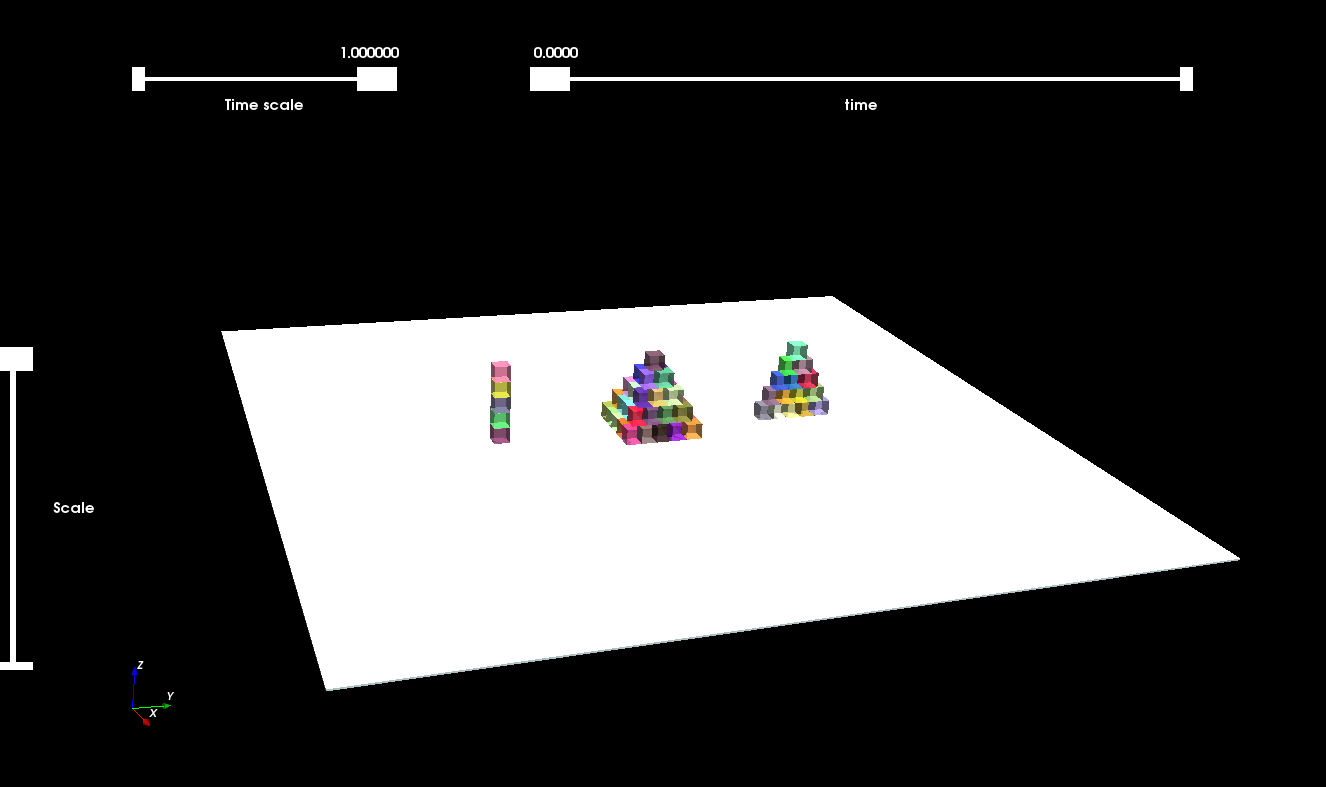
\includegraphics[scale=0.2]{Results/Example/cubes.png}
\caption{Box Stacks, set of examples in the comparison.}
\end{figure}
\end{frame}

\begin{frame}{Performance profiles}
For a set $P$ of $n_{p}$ problems, and a set $S$ of $n_{s}$ solvers, we define a performance criterion for a solver $s$, a problem $p$ and a required precision \textit{tol} by
\begin{align}
	t_{p,s} = \text{computing time required for } s \text{ to solve } p \text{ at precision \textit{tol}}
\end{align}
A performance ratio over all the solvers is defined by
\begin{align}
	r_{p,s} = \frac{t_{p,s}}{\min \lbrace t_{p,s}, s \in S \rbrace} \geq 1
\end{align}
For $\tau > 1$, we define a distribution function $\rho_{s}$ for the performance ratio for a solvers as
\begin{align}
	\rho_{s}(\tau) = \frac{1}{n_{p}} card \lbrace p \in P, r_{p,s} \leq \tau \rbrace \leq 1
\end{align}
%This distribution computes the number of problems $p$ that are solved with a performance ratio below a given threshold $\tau$. In other words, $\rho_{s}(\tau)$ represents the probability that the solver $s$ has a performance ratio not larger than a factor $\tau$ of the best solver. It is worth noting that $\rho_{s}(1)$ represents the probability that the solver $s$ beats the other solvers, and $\rho_{s}(\tau)$ characterizes the robustness of the method for large values of $\tau$. To summarize: the higher $\rho_{s}$ is, the better the method is. In the sequel, the term performance profile denotes a graph of the functions $\rho_{s}(\tau)$, $\tau > 1$. The computational time is used to measure performance in the algorithms.
\end{frame}

\section{Results}
%In this section, we perform a comparison of the algorithms by family of optimal penalty parameter. The goal is to study the influence of the various parameters and possible strategies on the performance of the solvers.
\begin{frame}
Family of optimal penalty parameters
\begin{itemize}
\item Ghadimi
\item Di Cairano
\item Acary
\item Normal
\end{itemize}
\end{frame}

\subsection{Ghadimi}
\begin{frame}{Ghadimi}
\begin{figure}[hbtp]
\centering
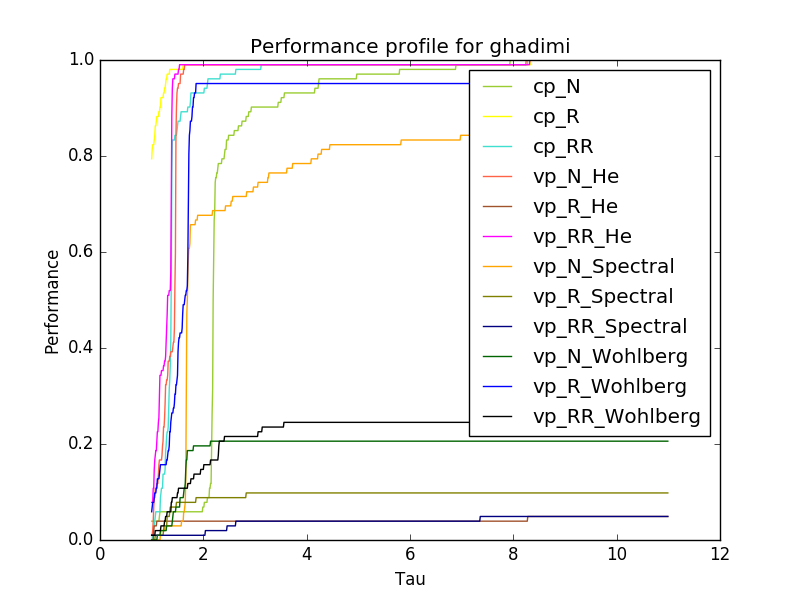
\includegraphics[scale=0.4]{Results/Ghadimi_mini.png}
\caption{Comparison of algorithms for Ghadimi optimal penalty parameter.}
\end{figure}
\end{frame}

\subsection{Di Cairano}
\begin{frame}{Di Cairano}
\begin{figure}[hbtp]
\centering
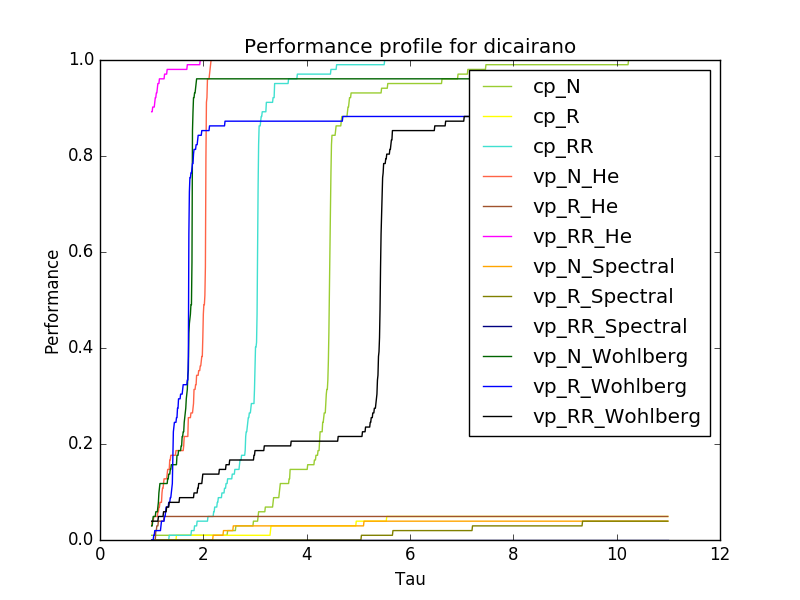
\includegraphics[scale=0.4]{Results/DiCairano_mini.png}
\caption{Comparison of algorithms for Di Cairano optimal penalty parameter.}
\end{figure}
\end{frame}

\subsection{Acary}
\begin{frame}{Acary}
\begin{figure}[hbtp]
\centering
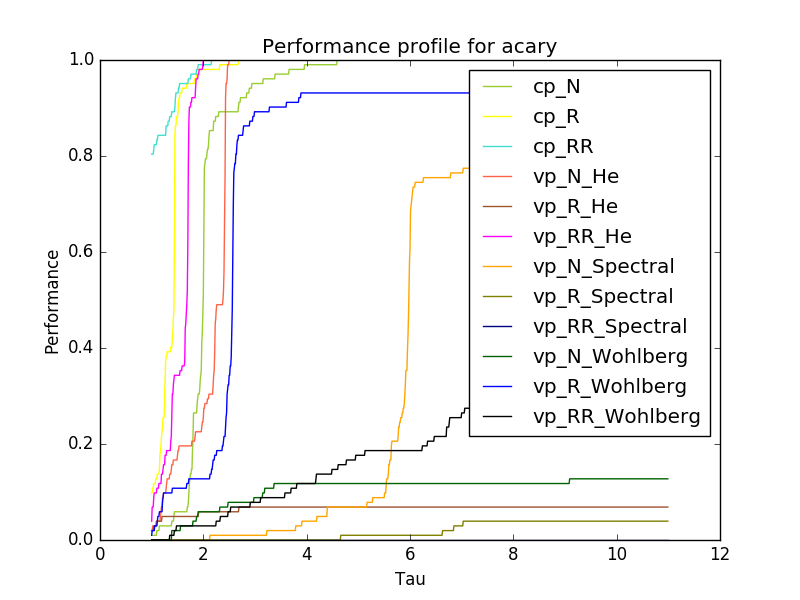
\includegraphics[scale=0.4]{Results/Acary_mini.png}
\caption{Comparison of algorithms for Acary optimal penalty parameter.}
\end{figure}
\end{frame}

\subsection{Normal}
\begin{frame}{Normal}
\begin{figure}[hbtp]
\centering
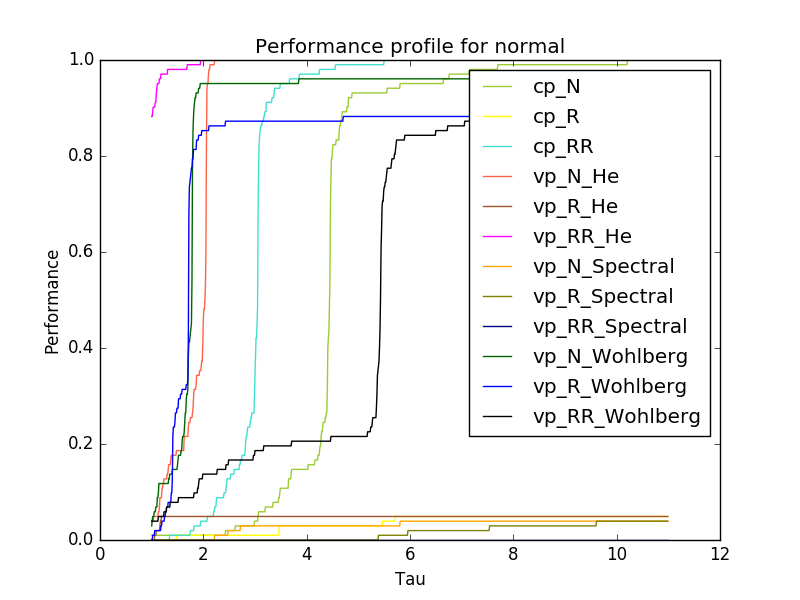
\includegraphics[scale=0.4]{Results/Normal_mini.png}
\caption{Comparison of algorithms for Normal optimal penalty parameter.}
\end{figure}
\end{frame}

\subsection{Discussion}
\begin{frame}{Discussion}
In Table \ref{Table:2} are depicted the best algorithms with their respective optimal penalty parameter. Although their behavior are very close, Di Cairano takes into account the data size of the problem, which makes it a more general solver.

\begin{table}[h!]
\resizebox{\textwidth}{!}{
\centering
 \begin{tabular}{||c c c||} 
 \hline
  & vp-RR-He \eqref{alg:prototype.vp-RR-He} (Di Cairano) & vp-RR-He \eqref{alg:prototype.vp-RR-He} (Normal) \\ [0.5ex] 
 \hline\hline
 $\rho_{s}(1)$ & 0.892 & 0.882 \\ 
 \hline
 $\tau_{\rho_{s} = 1}$ & 1.94 & 1.95 \\
 \hline
 Total CPU time (s) & 45.43 & 45.32 \\ [1ex] 
 \hline
\end{tabular}
}
\caption{Comparison of best algorithms.}
\label{Table:2}
\end{table}


It is worth noting that for the penalty parameter proposed in this work (Acary), its best performance is with cp-RR, i.e., this value is the closest one to the optimal and there is no need to update it under any scheme.
\end{frame}

\section{S-update}
\begin{frame}{S-update}
\begin{itemize}
\item External update
\item Internal update
\item Initial guess
\end{itemize}
\end{frame}

\subsection{Internal update}
\begin{frame}{Internal update}
For the next development, we consider
\begin{align}
	\Phi(\bi{u})
	= [\mu^{\alpha} \| E_{t} \bi{u}^{\alpha} \| \hat{\bi{e}}_{n}, \alpha = 1...n_{c}]^{T}
	= [\mu^{\alpha} \| E_{t} \left( H \bi{v} + \bi{w} \right)^{\alpha} \| \hat{\bi{e}}_{t}, \alpha = 1...n_{c}]^{T}
\end{align}
therefore $\Phi(\bi{u})$ could be seen as $\Phi(\bi{v})$. Then, the problem \eqref{eq.ADMM.friction.AugLagrange} is a minimization problem of a convex 
function under non-linear equality constraints. 
Its augmented Lagrangian is formulated as 
\begin{align}
  L_{\rho}(\bi{v};\tilde{\bi{u}};\bi{\zeta}) 
  =& \frac{1}{2} \bi{v}^{\top} M \bi{v} + \bi{f}^{\top} \bi{v} 
  +  \delta_{K_{e,\mu}^{*}}(\tilde{\bi{u}}) +  \frac{\rho}{2} 
  \| H \bi{v} + \bi{w} + \Phi(\bi{v}) + \bi{\zeta}  - \tilde{\bi{u}} \|^{2}
    - \frac{\rho}{2} \| \bi{\zeta}\|^{2} 
\end{align}
where $\rho$ is the penalty parameter, and $\bi{\zeta} \in \Re^{m}$ is  the scaled dual variable. The ADMM solving problem \eqref{P.quadratic.SOCP.2} consists of 
iterating the updates 
\begin{align}
  \bi{v}^{k+1} 
  &:= \argmin_{\bi{v}} 
  L_{\rho}(\bi{v};\tilde{\bi{u}}^{k};\bi{\zeta}^{k})   
  \label{eq.ADMM.friction.1.1new} \\
  \tilde{\bi {u}}^{k+1}
  &:= \argmin_{\tilde{\bi{u}}} 
    L_{\rho}(\bi{v}^{k+1};\tilde{\bi{u}};\bi{\zeta}^{k}) 
    \label{eq.ADMM.friction.1.2new} \\
  \bi{\zeta}^{k+1} &:= \bi{\zeta}^{k} 
  + 
  H \bi{v}^{k+1} - \tilde{\bi{u}}^{k+1} + \Phi(\bi{v}^{k+1})  
  \label{eq.ADMM.friction.1.3bis}
\end{align}
\end{frame}

\begin{frame}{Internal update}
\begin{itemize}
\item $v$-update
\end{itemize}
The first step in \eqref{eq.ADMM.friction.1.1new} corresponds to 
unconstrained minimization of a convex function. 
It follows from the stationarity condition of this convex 
function that $\bi{v}^{k+1}$ is the solution to the following system of 
non-linear equations: 
\begin{align}
  \Bigl[ M + 
  \rho \left( H^{\top} + \partial_{\bi{v}} \Phi(\bi{v}^{k+1}) \right) H \Bigr] \bi{v}^{k+1} 
  = -\bi{f} 
  + \rho \left( H^{\top} + \partial_{\bi{v}} \Phi(\bi{v}^{k+1}) \right) (\tilde{\bi{u}}^k - \bi{w} - \Phi(\bi{v}^{k+1}) - \bi{\zeta}^k)
\end{align}
this non-linearity is difficult to handle, however, if the previous iteration is considered in the $\Phi(\bi{v})$ term, we get the following system of linear equations
\begin{align}
  \Bigl[ M + 
  \rho \left( H^{\top} + \partial_{\bi{v}} \Phi(\bi{v}^{k}) \right) H \Bigr] \bi{v}^{k+1} 
  = -\bi{f} 
  + \rho \left( H^{\top} + \partial_{\bi{v}} \Phi(\bi{v}^{k}) \right) (\tilde{\bi{u}}^k - \bi{w} - \Phi(\bi{v}^{k}) - \bi{\zeta}^k)
\end{align}
which follows the same structure of \eqref{eq.ADMM.friction.2.1} and allows us to perform a LU or Cholesky factorization. If $\| E_{t} \bi{u}^{\alpha} \| \neq 0$
\begin{align}
  \partial_{\bi{v}} \Phi(\bi{v})
  = \Bigl[ \mu^{\alpha} \hat{\bi{e}}_{n}^{\top}
  \frac{E_{t} \left( H \bi{v} + \bi{w} \right)^{\alpha}}{\| E_{t} \left( H \bi{v} + \bi{w} \right)^{\alpha} \|}
  E_{t}^{\top} H^{\alpha^{\top}}, \alpha = 1...n_{c} \Bigr]^{T} = \Psi
\end{align}
\end{frame}

\begin{frame}{Internal update}
Therefore
\begin{align}
  \Bigl[ M + 
  \rho \left( H^{\top} + \Psi \right) H \Bigr] \bi{v}^{k+1} 
  = -\bi{f} 
  + \rho \left( H^{\top} + \Psi \right) (\tilde{\bi{u}}^k - \bi{w} - \Phi(\bi{v}^{k}) - \bi{\zeta}^k)  
  \label{eq.ADMM.subgradient0}
\end{align}
Note that if in \eqref{eq.ADMM.friction.1.1new} it is evaluated $\Phi(\bi{v})$ in the previous iteration before compute the stationary condition, it results in
\begin{align}
  \Bigl[ M + 
  \rho H^{\top} H \Bigr] \bi{v}^{k+1} 
  = -\bi{f} 
  + \rho H^{\top} (\tilde{\bi{u}}^k - \bi{w} - \Phi(\bi{v}^{k}) - \bi{\zeta}^k) 
  \label{eq.ADMM.subgradient1}
\end{align}
which is a pseudo-update of \eqref{eq.ADMM.friction.1.1new} in comparison with \eqref{eq.ADMM.subgradient0}, but it aims to be faster whitout the compuation of $\Psi$, therefore, \eqref{eq.ADMM.subgradient1} will be used.

\begin{itemize}
\item $\tilde{u}$-update
\end{itemize}
The second step in \eqref{eq.ADMM.friction.1.2new} can be computed independently for each $\alpha = 1 ... n_{c}$ as 
\begin{align}
  \tilde{\bi{u}}^{k+1}
  &:= \argmin_{\tilde{\bi{u}}} 
    \delta_{K_{e,\mu}^{*}}(\tilde{\bi{u}}) 
    + \frac{\rho}{2} 
    \| H \bi{v}^{k+1} + \bi{w} + \Phi(\bi{v}^{k}) + \bi{\zeta}^{k} - \bi{\tilde u} \|^{2}
  \label{eq.ADMM.friction.2.2bis}
\end{align}
\eqref{eq.ADMM.friction.2.2bis} can be rewritten by using the projection 
onto the second-order cone as 
\begin{align}
  \tilde{\bi{u}}^{k+1} := \Pi_{K_{e,\mu}^{*}}(H \bi{v}^{k+1} + \bi{w} + \bi{\zeta}^{k} + \Phi(\bi{v}^{k+1}))
\end{align}
\end{frame}

\begin{frame}{S-update}
\begin{itemize}
\item External update
\end{itemize}
In this case, the external error measurement is given for each $\alpha = 1 ... n_{c}$ by 
\begin{align}
	\Bigl[ \frac{\Phi(\bi{v}^{k+1}) - \Phi(\bi{v}^{k})}{\Phi(\bi{v}^{k})} \Bigr]^{\alpha} \leq \epsilon^{ext} \label{eq.stopcriterionexternal}
\end{align}
where $\epsilon^{ext}$ is the external tolerance, with a value $10^{-3}$.

\begin{itemize}
\item SICONOS error
\end{itemize}
The primal residual measures the error in the constraint in \eqref{CF.complementary}, but also the error could be measured from the dynamic equation and the natural map \eqref{eq.ADMM.naturalmap} as
\begin{align}
\epsilon^{SIC} = \sqrt{\| M \bi{v} + \bi{f} - H^{\top} \bi{r} \|^{2} + \| \tilde{\bi{u}} - \Pi_{K_{e,\mu}^{*}}(\tilde{\bi{u}} - \rho \bi{r}) \|^{2}}
\end{align}
\end{frame}

\section{Numerical experience: S-update}
%In most of the test examples the behavior dispicted in Figure 5-7 is observed.
%This is analyzed with the best solver of Section 7 and the test example \emph{Box Stacks-i1000-352-6}.

\begin{frame}{External S-update}
%In Figure 5 is observed a convergence after 7 external iterations. Note that the first value is not shown because is zero.
\begin{figure}[hbtp]
\centering
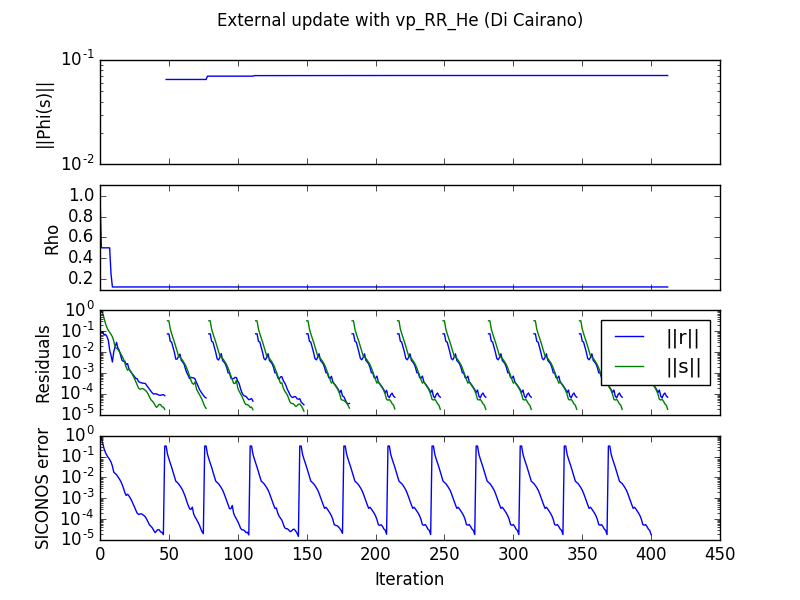
\includegraphics[scale=0.4]{Results/S_update/External13.png}
\caption{External update with vp-RR-He (Di Cairano).}
\end{figure}
\end{frame}

\begin{frame}{Internal S-update}
%In Figure 6 is observed a convergence after 43 internal iterations. From iteration 25 the same value holds, but the stop criterion \eqref{eq.stopcriterion} is not satisfied.
\begin{figure}[hbtp]
\centering
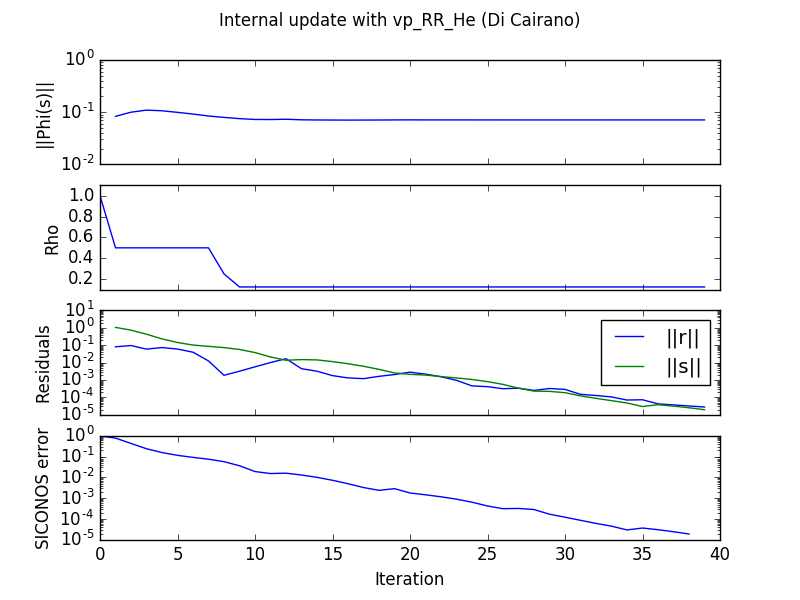
\includegraphics[scale=0.4]{Results/S_update/Internal13.png}
\caption{Internal update with vp-RR-He (Di Cairano).}
\end{figure}
\end{frame}

\begin{frame}{Internal S-update}
%In Figure 7 is despicted the same internal update, but the stop criterion \eqref{eq.stopcriterion} is changed for the external one  \eqref{eq.stopcriterionexternal}. It is observed that $\| \Phi(\bi{v}) \|$ holds from iteration 25, but $\Phi(\bi{v})^{\alpha}$ is not the same from iteration to iteration.
\begin{figure}[hbtp]
\centering
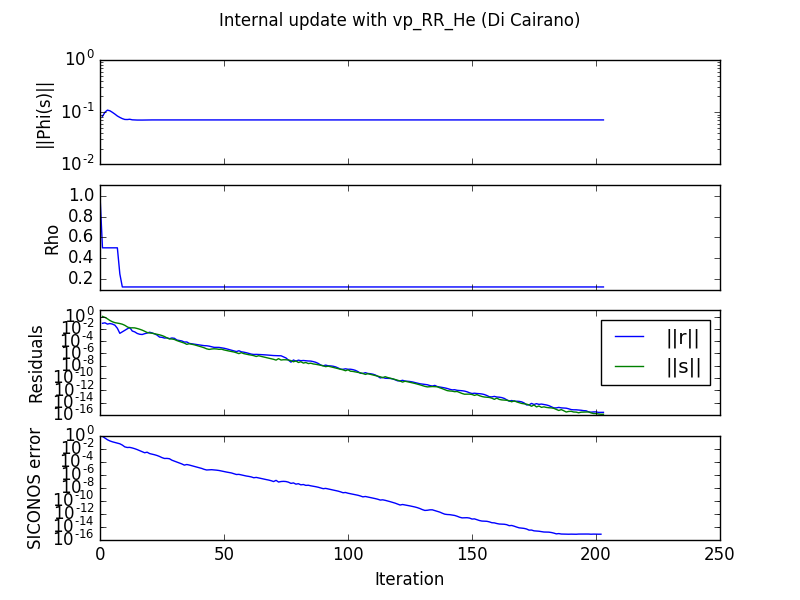
\includegraphics[scale=0.4]{Results/S_update/Internal13outsidestop.png}
\caption{Internal update with vp-RR-He (Di Cairano) and stop criterion in \eqref{eq.stopcriterionexternal}.}
\end{figure}
\end{frame}

\begin{frame}{Discussion}
In Table \ref{Table:3} are shown the values of the final $\| \Phi(s) \|$ with its respectives first and last contact vector $\Phi(s)^{\alpha}$:
\begin{table}[h!]
\resizebox{\textwidth}{!}{
\centering
 \begin{tabular}{||c c c c||} 
 \hline
  & External & Internal & Internal-s \\ [0.5ex] 
 \hline\hline
 $\| \Phi(s) \|$ & 7.10e-02 & 7.10e-02 & 7.10e-02 \\ 
 \hline
 $\Phi(s)^{\alpha = 1}$ & [8.31e-06  0.00e+00  0.00e+00] & [6.49e-06  0.00e+00  0.00e+00] & [7.45e-06  0.00e+00  0.00e+00] \\
 \hline
 $\Phi(s)^{\alpha = n_{c}}$ & [1.02e-05  0.00e+00  0.00e+00] & [1.19e-05  0.00e+00  0.00e+00] & [7.85e-06  0.00e+00  0.00e+00] \\ [1ex] 
 \hline
\end{tabular}
}
\caption{Comparison of s-update}
\label{Table:3}
\end{table}

%Both external and internal update converges to the same value of $\| \Phi(s) \|$, but this is an apparent result of uniqueness when $\Phi(s)^{\alpha}$ is compared in each case. Therefore, the internal update does not guarantee the same result for $\Phi(s)$. However, all of them have low values of SICONOS error and residuals, i.e., they solve the problem \eqref{CF.complementary}. This opens the question if these aproaches converge at some level to a different solutions of problem \eqref{CF.complementary}.
\end{frame}

\section{Final remarks}
\begin{frame}{Final remarks}
\begin{itemize}
\item The best improvement is given by vp-RR-He with Di Cairano and Normal optimal penalty parameter.
\item Open question in the same numerical value of convergence in  $\Phi(s)$ with external and internal update.
\item Comparison with other numerical methods (Fixed point and projection methods for VI formulation, Newton based methods, Splitting techniques and proximal point algorithm, etc.).
\end{itemize}
\end{frame}

\begin{frame}[allowframebreaks]
\frametitle{References}
\bibliographystyle{unsrt}
\bibliography{myreferences}
\end{frame}

\section*{Appendix A. ADMM algorithms}

\subsection{Constant penalty parameter}
\begin{frame}{Constant penalty parameter}
The relaxed ADMM involves a parameter $\eta \in (0,1)$. It is desirible to restart the method as infrequently as possible, it is recommended a value of $\eta$ close to $1$ \citep{goldstein2014fast}. In our case $\eta = 0.999$ was used.

\begin{algorithm}[H]
  \scriptsize
  \caption{ADMM.}
  \label{alg:prototype.cp-N}
  \begin{algorithmic}[1]
    \Require
    $\bi{y}^{0}$, $\bi{z}^{0}$, and $\rho > 0$ 
    \For{$k=0,1,2,\dots$}
    \State
    $\bi{x}^{k+1} 
    := \argmin_{\bi{x}} L_{\rho}(\bi{x};\bi{y}^{k};{\bi{z}}^{k})$ 
    \State
    $\bi{y}^{k+1} 
    := \argmin_{\bi{y}} L_{\rho}(\bi{x}^{k+1};\bi{y};{\bi{z}}^{k})$ 
    \State
    $\bi{z}^{k+1} 
  := \bi{z}^{k} + A \bi{x}^{k+1} + B \bi{y}^{k+1} - \bi{c}$ 
    \State
    Stop criterion in \eqref{eq.stopcriterion}
    \EndFor
  \end{algorithmic}
\end{algorithm}
\end{frame}

\begin{frame}{Constant penalty parameter}
\begin{algorithm}[H]
  \scriptsize
  \caption{Relaxed ADMM.}
  \label{alg:prototype.cp-R}
  \begin{algorithmic}[1]
    \Require
    $\bi{y}^{0} = \hat{\bi{y}}^{0}$, $\bi{z}^{0}=\hat{\bi{z}}^{0}$, $\alpha_{0}=1$, and $\rho > 0$ 
    \For{$k=0,1,2,\dots$}
    \State
    $\bi{x}^{k+1} 
    := \argmin_{\bi{x}} L_{\rho}(\bi{x};\hat{\bi{y}}^{k};\hat{\bi{z}}^{k})$ 
    \State
    $\bi{y}^{k+1} 
    := \argmin_{\bi{y}} L_{\rho}(\bi{x}^{k+1};\bi{y};\hat{\bi{z}}^{k})$ 
    \State
    $\bi{z}^{k+1} 
  := \bi{z}^{k} + A \bi{x}^{k+1} + B \bi{y}^{k+1} - \bi{c}$ 
    \State
    Stop criterion in \eqref{eq.stopcriterion}
    \State
    Relaxation in \eqref{eq.ADMM.relaxed}
    \EndFor
  \end{algorithmic}
\end{algorithm}

%\refalg{alg:fast.ADMM.restart.prototype}. 
\begin{algorithm}[H]
  \scriptsize
  \caption{Relaxed + Restart ADMM.}
  \label{alg:prototype.cp-RR}
  \begin{algorithmic}[1]
    \Require
    $\bi{y}^{0} = \hat{\bi{y}}^{0}$, $\bi{z}^{0}=\hat{\bi{z}}^{0}$, 
    $\alpha_{0}=1$, $\eta \approx 1$, and $\rho > 0$ 
    \For{$k=0,1,2,\dots$}
    \State
    $\bi{x}^{k+1} 
    := \argmin_{\bi{x}} L_{\rho}(\bi{x};\hat{\bi{y}}^{k};\hat{\bi{z}}^{k})$ 
    \State
    $\bi{y}^{k+1} 
    := \argmin_{\bi{y}} L_{\rho}(\bi{x}^{k+1};\bi{y};\hat{\bi{z}}^{k})$ 
    \State
    $\bi{z}^{k+1} 
  := \bi{z}^{k} + A \bi{x}^{k+1} + B \bi{y}^{k+1} - \bi{c}$ 
    \State
    Stop criterion in \eqref{eq.stopcriterion} 
    \State
	Relaxation + Restart in \eqref{eq.ADMM.relaxed} \eqref{eq.ADMM.restart}
    \EndFor
  \end{algorithmic}
\end{algorithm}
\end{frame}

\subsection{Varying penalty parameter - He}
\begin{frame}{Varying penalty parameter - He}
In Wang et al. the value $\tau = 2$ generally performs well in the $\rho$ update \citep{WANG2001}.

\begin{algorithm}[H]
  \scriptsize
  \caption{ADMM.}
  \label{alg:prototype.vp-N-He}
  \begin{algorithmic}[1]
    \Require
    $\bi{y}^{0}$, $\bi{z}^{0}$, $\varphi = 10$, $\tau = 2$, and $\rho > 0$ 
    \For{$k=0,1,2,\dots$}
    \State
    $\bi{x}^{k+1} 
    := \argmin_{\bi{x}} L_{\rho}(\bi{x};{\bi{y}}^{k};{\bi{z}}^{k})$ 
    \State
    $\bi{y}^{k+1} 
    := \argmin_{\bi{y}} L_{\rho}(\bi{x}^{k+1};\bi{y};{\bi{z}}^{k})$ 
    \State
    $\bi{z}^{k+1} 
  := \frac{\rho^{k-1}}{\rho^{k}} \left( \bi{z}^{k} + A \bi{x}^{k+1} + B \bi{y}^{k+1} - \bi{c} \right)$ 
    \State
    Stop criterion in \eqref{eq.stopcriterion}
    \State
    Update of $\rho$ in (He)
    \EndFor
  \end{algorithmic}
\end{algorithm}
\end{frame}

\begin{frame}{Varying penalty parameter - He}
\begin{algorithm}[H]
  \scriptsize
  \caption{Relaxed ADMM.}
  \label{alg:prototype.vp-R-He}
  \begin{algorithmic}[1]
    \Require
    $\bi{y}^{0} = \hat{\bi{y}}^{0}$, $\bi{z}^{0}=\hat{\bi{z}}^{0}$, $\alpha_{0}=1$, $\varphi = 10$, $\tau = 2$, and $\rho > 0$ 
    \For{$k=0,1,2,\dots$}
    \State
    $\bi{x}^{k+1} 
    := \argmin_{\bi{x}} L_{\rho}(\bi{x};\hat{\bi{y}}^{k};\hat{\bi{z}}^{k})$ 
    \State
    $\bi{y}^{k+1} 
    := \argmin_{\bi{y}} L_{\rho}(\bi{x}^{k+1};\bi{y};\hat{\bi{z}}^{k})$ 
    \State
    $\bi{z}^{k+1} 
  := \frac{\rho^{k-1}}{\rho^{k}} \left( \bi{z}^{k} + A \bi{x}^{k+1} + B \bi{y}^{k+1} - \bi{c} \right)$ 
    \State
    Stop criterion in \eqref{eq.stopcriterion}
    \State
    Relaxation in \eqref{eq.ADMM.relaxed}
    \State
    Update of $\rho$ in (He)
    \EndFor
  \end{algorithmic}
\end{algorithm}

%\refalg{alg:fast.ADMM.restart.prototype}. 
\begin{algorithm}[H]
  \scriptsize
  \caption{Relaxed + Restart ADMM.}
  \label{alg:prototype.vp-RR-He}
  \begin{algorithmic}[1]
    \Require
    $\bi{y}^{0} = \hat{\bi{y}}^{0}$, $\bi{z}^{0}=\hat{\bi{z}}^{0}$, 
    $\alpha_{0}=1$, $\eta \approx 1$, $\varphi = 10$, $\tau = 2$, and $\rho > 0$ 
    \For{$k=0,1,2,\dots$}
    \State
    $\bi{x}^{k+1} 
    := \argmin_{\bi{x}} L_{\rho}(\bi{x};\hat{\bi{y}}^{k};\hat{\bi{z}}^{k})$ 
    \State
    $\bi{y}^{k+1} 
    := \argmin_{\bi{y}} L_{\rho}(\bi{x}^{k+1};\bi{y};\hat{\bi{z}}^{k})$ 
    \State
    $\bi{z}^{k+1} 
  := \frac{\rho^{k-1}}{\rho^{k}} \left( \bi{z}^{k} + A \bi{x}^{k+1} + B \bi{y}^{k+1} - \bi{c} \right)$ 
    \State
    Stop criterion in \eqref{eq.stopcriterion}
    \State
    Relaxation + Restart in \eqref{eq.ADMM.relaxed} \eqref{eq.ADMM.restart}
    \State
    Update of $\rho$ in (He)
    \EndFor
  \end{algorithmic}
\end{algorithm}
\end{frame}

\subsection{Varying penalty parameter - Wohlberg}
\begin{frame}{Varying penalty parameter - Wohlberg}
In He et al. the value $\tau_{max} = 100$ generally performs well in the $\rho$ update \citep{wohlberg2017admm}.

\begin{algorithm}[H]
  \scriptsize
  \caption{ADMM.}
  \label{alg:prototype.vp-N-Wohlberg}
  \begin{algorithmic}[1]
    \Require
    $\bi{y}^{0}$, $\bi{z}^{0}$, $\xi = 1$, $\varphi = 10$, $\tau_{max} = 100$, and $\rho > 0$ 
    \For{$k=0,1,2,\dots$}
    \State
    $\bi{x}^{k+1} 
    := \argmin_{\bi{x}} L_{\rho}(\bi{x};{\bi{y}}^{k};{\bi{z}}^{k})$ 
    \State
    $\bi{y}^{k+1} 
    := \argmin_{\bi{y}} L_{\rho}(\bi{x}^{k+1};\bi{y};{\bi{z}}^{k})$ 
    \State
    $\bi{z}^{k+1} 
  := \frac{\rho^{k-1}}{\rho^{k}} \left( \bi{z}^{k} + A \bi{x}^{k+1} + B \bi{y}^{k+1} - \bi{c} \right)$ 
    \State
    Stop criterion in \eqref{eq.stopcriterion}
    \State
    Update of $\rho$ in (Wohlberg)
    \EndFor
  \end{algorithmic}
\end{algorithm}
\end{frame}

\begin{frame}{Varying penalty parameter - Wohlberg}
\begin{algorithm}[H]
  \scriptsize
  \caption{Relaxed ADMM.}
  \label{alg:prototype.vp-R-Wohlberg}
  \begin{algorithmic}[1]
    \Require
    $\bi{y}^{0} = \hat{\bi{y}}^{0}$, $\bi{z}^{0}=\hat{\bi{z}}^{0}$, $\alpha_{0}=1$, $\xi = 1$, $\varphi = 10$, $\tau_{max} = 100$, and $\rho > 0$ 
    \For{$k=0,1,2,\dots$}
    \State
    $\bi{x}^{k+1} 
    := \argmin_{\bi{x}} L_{\rho}(\bi{x};\hat{\bi{y}}^{k};\hat{\bi{z}}^{k})$ 
    \State
    $\bi{y}^{k+1} 
    := \argmin_{\bi{y}} L_{\rho}(\bi{x}^{k+1};\bi{y};\hat{\bi{z}}^{k})$ 
    \State
    $\bi{z}^{k+1} 
  := \frac{\rho^{k-1}}{\rho^{k}} \left( \bi{z}^{k} + A \bi{x}^{k+1} + B \bi{y}^{k+1} - \bi{c} \right)$ 
    \State
    Stop criterion in \eqref{eq.stopcriterion}
    \State
    Relaxation in \eqref{eq.ADMM.relaxed}
    \State
    Update of $\rho$ in (Wohlberg)
    \EndFor
  \end{algorithmic}
\end{algorithm}

%\refalg{alg:fast.ADMM.restart.prototype}. 
\begin{algorithm}[H]
  \scriptsize
  \caption{Relaxed + Restart ADMM.}
  \label{alg:prototype.vp-RR-Wohlberg}
  \begin{algorithmic}[1]
    \Require
    $\bi{y}^{0} = \hat{\bi{y}}^{0}$, $\bi{z}^{0}=\hat{\bi{z}}^{0}$, 
    $\alpha_{0}=1$, $\eta \approx 1$, $\xi = 1$, $\varphi = 10$, $\tau_{max} = 100$, and $\rho > 0$ 
    \For{$k=0,1,2,\dots$}
    \State
    $\bi{x}^{k+1} 
    := \argmin_{\bi{x}} L_{\rho}(\bi{x};\hat{\bi{y}}^{k};\hat{\bi{z}}^{k})$ 
    \State
    $\bi{y}^{k+1} 
    := \argmin_{\bi{y}} L_{\rho}(\bi{x}^{k+1};\bi{y};\hat{\bi{z}}^{k})$ 
    \State
    $\bi{z}^{k+1} 
  := \frac{\rho^{k-1}}{\rho^{k}} \left( \bi{z}^{k} + A \bi{x}^{k+1} + B \bi{y}^{k+1} - \bi{c} \right)$ 
    \State
    Stop criterion in \eqref{eq.stopcriterion}
    \State
    Relaxation + Restart in \eqref{eq.ADMM.relaxed} \eqref{eq.ADMM.restart}
    \State
    Update of $\rho$ in (Wohlberg)
    \EndFor
  \end{algorithmic}
\end{algorithm}
\end{frame}

\subsection{Varying penalty parameter - Spectral}
\begin{frame}{Varying penalty parameter - Spectral}
Xu et al. suggest only updating the stepsize every $T_{f}$ iterations. Safeguarding threshold $\epsilon^{cor} = 0.2$ and $T_{f} = 2$ generally perform well \citep{xu2016adaptive}.

\begin{algorithm}[H]
  \scriptsize
  \caption{ADMM.}
  \label{alg:prototype.vp-N-Spectral}
  \begin{algorithmic}[1]
    \Require
    $\bi{y}^{0}$, $\bi{z}^{0}$, $T_{f} = 2$, $\epsilon^{cor} = 0.2$, and $\rho > 0$ 
    \For{$k=0,1,2,\dots$}
    \State
    $\bi{x}^{k+1} 
    := \argmin_{\bi{x}} L_{\rho}(\bi{x};{\bi{y}}^{k};{\bi{z}}^{k})$ 
    \State
    $\bi{y}^{k+1} 
    := \argmin_{\bi{y}} L_{\rho}(\bi{x}^{k+1};\bi{y};{\bi{z}}^{k})$ 
    \State
    $\bi{z}^{k+1} 
  := \frac{\rho^{k-1}}{\rho^{k}} \left( \bi{z}^{k} + A \bi{x}^{k+1} + B \bi{y}^{k+1} - \bi{c} \right)$ 
    \State
    Stop criterion in \eqref{eq.stopcriterion}
    \If{$mod(k,T_{f}) = 1$}
    \State
    Update of $\rho$ in (Spectral)
    \Else
    \State
    $\rho^{k+1} \leftarrow \rho^{k}$
    \EndIf
    \EndFor
  \end{algorithmic}
\end{algorithm}
\end{frame}

\begin{frame}{Varying penalty parameter - Spectral}
\begin{algorithm}[H]
  \scriptsize
  \caption{Relaxed ADMM.}
  \label{alg:prototype.vp-R-Spectral}
  \begin{algorithmic}[1]
    \Require
    $\bi{y}^{0} = \hat{\bi{y}}^{0}$, $\bi{z}^{0}=\hat{\bi{z}}^{0}$, $\alpha_{0}=1$, $T_{f} = 2$, $\epsilon^{cor} = 0.2$, and $\rho > 0$ 
    \For{$k=0,1,2,\dots$}
    \State
    $\bi{x}^{k+1} 
    := \argmin_{\bi{x}} L_{\rho}(\bi{x};\hat{\bi{y}}^{k};\hat{\bi{z}}^{k})$ 
    \State
    $\bi{y}^{k+1} 
    := \argmin_{\bi{y}} L_{\rho}(\bi{x}^{k+1};\bi{y};\hat{\bi{z}}^{k})$ 
    \State
    $\bi{z}^{k+1} 
  := \frac{\rho^{k-1}}{\rho^{k}} \left( \bi{z}^{k} + A \bi{x}^{k+1} + B \bi{y}^{k+1} - \bi{c} \right)$ 
    \State
    Stop criterion in \eqref{eq.stopcriterion}
    \State
    Relaxation in \eqref{eq.ADMM.relaxed}
    \If{$mod(k,T_{f}) = 1$}
    \State
    Update of $\rho$ in (Spectral)
    \Else
    \State
    $\rho^{k+1} \leftarrow \rho^{k}$
    \EndIf
    \EndFor
  \end{algorithmic}
\end{algorithm}

%\refalg{alg:fast.ADMM.restart.prototype}. 
\begin{algorithm}[H]
  \scriptsize
  \caption{Relaxed + Restart ADMM.}
  \label{alg:prototype.vp-RR-Spectral}
  \begin{algorithmic}[1]
    \Require
    $\bi{y}^{0} = \hat{\bi{y}}^{0}$, $\bi{z}^{0}=\hat{\bi{z}}^{0}$, 
    $\alpha_{0}=1$, $\eta \approx 1$, $T_{f} = 2$, $\epsilon^{cor} = 0.2$, and $\rho > 0$ 
    \For{$k=0,1,2,\dots$}
    \State
    $\bi{x}^{k+1} 
    := \argmin_{\bi{x}} L_{\rho}(\bi{x};\hat{\bi{y}}^{k};\hat{\bi{z}}^{k})$ 
    \State
    $\bi{y}^{k+1} 
    := \argmin_{\bi{y}} L_{\rho}(\bi{x}^{k+1};\bi{y};\hat{\bi{z}}^{k})$ 
    \State
    $\bi{z}^{k+1} 
  := \frac{\rho^{k-1}}{\rho^{k}} \left( \bi{z}^{k} + A \bi{x}^{k+1} + B \bi{y}^{k+1} - \bi{c} \right)$ 
    \State
    Stop criterion in \eqref{eq.stopcriterion}
    \State
    Relaxation + Restart in \eqref{eq.ADMM.relaxed} \eqref{eq.ADMM.restart}
    \If{$mod(k,T_{f}) = 1$}
    \State
    Update of $\rho$ in (Spectral)
    \Else
    \State
    $\rho^{k+1} \leftarrow \rho^{k}$
    \EndIf
    \EndFor
  \end{algorithmic}
\end{algorithm}
\end{frame}

\end{document}
%%% Local Variables: 
%%% mode: latex
%%% TeX-master: t
%%% End: 
